\documentclass{article}
\usepackage[paperwidth=84.1cm,paperheight=118.9cm,margin=0cm]{geometry}
\usepackage{fontspec}
\usepackage{unicode-math}
\usepackage[brazilian]{babel}
\usepackage{graphicx}
\usepackage{tikz}
\usetikzlibrary{arrows.meta}
\usepackage{qrcode}
\usepackage[hidelinks]{hyperref}
\setmainfont{Arial}
\setsansfont{Arial}
\setmathfont{latinmodern-math.otf}
\hypersetup{pdftitle={ALGORITMOS EXATOS PARA O PROBLEMA DE VISITA DE POLÍGONOS},pdfauthor={Gabriel Freire Ushijima; Ernesto G. Birgin},pdfsubject={34º SIICUSP, IME-USP}}
\pagestyle{empty}
\setlength{\parindent}{0pt}
\setlength{\parskip}{0.24em}
\definecolor{Ink}{HTML}{142D38}
\definecolor{Muted}{HTML}{47616A}
\definecolor{Accent}{HTML}{CF5A20}
\definecolor{Pale}{HTML}{EEF4F1}
\definecolor{Rule}{HTML}{C5D3CF}
\definecolor{MapDark}{HTML}{102C38}
\definecolor{Route}{HTML}{FFAD66}
\definecolor{FirstVisit}{HTML}{81D864}
\definecolor{LastVisit}{HTML}{1F7A73}
\newsavebox{\posterbox}
% Named, measured blocks make overflow checks reproducible after each edit.
\newcommand{\block}[5]{%
  \node[anchor=north west,inner sep=0] at (#2,#3) {%
  \sbox{\posterbox}{\begin{minipage}[t]{#4cm}\raggedright #5\end{minipage}}%
  \typeout{POSTERBLOCK #1 x=#2 y=#3 w=#4 h=\the\dimexpr\ht\posterbox+\dp\posterbox\relax}%
  \usebox{\posterbox}};}
\newcommand{\head}[2]{{\sffamily\bfseries\fontsize{42}{48}\selectfont\color{Accent}#1\hspace{0.45cm}\color{Ink}#2\par}}
\newcommand{\bodytext}{\sffamily\mdseries\fontsize{30}{36}\selectfont\color{Ink}}
\newcommand{\smalltext}{\sffamily\mdseries\fontsize{25}{31}\selectfont\color{Muted}}
\newcommand{\tagtext}{\sffamily\bfseries\fontsize{25}{30}\selectfont\color{Accent}}
\newcommand{\metric}{\sffamily\bfseries\fontsize{66}{72}\selectfont\color{Accent}}
\begin{document}
\begin{tikzpicture}[remember picture,overlay,shift={(current page.north west)},x=1cm,y=-1cm]
  \fill[white] (0,0) rectangle (84.1,118.9);
  \fill[Ink] (0,0) rectangle (84.1,0.55);
  % Official title, identical to the submitted abstract.
  \block{event}{3}{2.0}{65}{\tagtext 34º SIICUSP\hspace{0.55cm}/\hspace{0.55cm}INSTITUTO DE MATEMÁTICA E ESTATÍSTICA\hspace{0.35cm}·\hspace{0.35cm}USP}
  \block{event-logo}{73.4}{1.9}{7.6}{
\includegraphics[width=\linewidth]{../resumo/assets/siicusp34-logo-pt.png}}
  \block{title}{3}{4.4}{69.5}{\sffamily\bfseries\fontsize{88}{96}\selectfont\color{Ink}ALGORITMOS EXATOS PARA O\\PROBLEMA DE VISITA DE POLÍGONOS}
  \block{subtitle}{3}{11.9}{78}{\sffamily\fontsize{34}{41}\selectfont\color{Muted}Geometria para escolher onde e em que ordem visitar regiões}
  \block{author}{3}{14.1}{37}{\sffamily\bfseries\fontsize{48}{55}\selectfont\color{Ink}Gabriel Freire Ushijima}
  \block{advisor}{42}{14.1}{39.1}{\sffamily\fontsize{38}{50}\selectfont\color{Ink}Orientador: \textbf{Ernesto G. Birgin}}
  \draw[Rule,line width=1.1pt] (3,17.0) -- (81.1,17.0);
  % Motivation; definitions precede both historical steps.
  \block{intro-head}{3}{18.3}{24.4}{\head{01}{A pergunta}}
  \block{intro}{3}{21.1}{24.4}{\bodytext Um drone parte do IME para fotografar institutos e outras regiões da USP. Precisamos escolher \textbf{a ordem das visitas e o ponto de contato} em cada região.}
  \block{question}{3}{27.3}{24.4}{\sffamily\bfseries\fontsize{37}{43}\selectfont\color{Ink}Qual é a menor rota que visita todas e retorna ao IME?}
  \draw[Accent,line width=2.2pt] (3,33.2) -- (6,33.2);
  \block{evolution}{3}{34.1}{24.4}{\smalltext\textbf{Do resumo à extensão.} O resumo apresentava o caso não convexo com ordem fixa. Após a submissão, concluímos a extensão para ordem livre.}
  \block{definitions-head}{30}{18.3}{51.1}{\head{02}{Dos pontos às regiões}}
  \block{tsp}{30}{21.5}{15.6}{\tagtext TSP\par\vspace{0.2cm}\bodytext Caixeiro viajante: menor ciclo que visita pontos. Escolhe a ordem.}
  \block{tpp}{47.2}{21.5}{15.6}{\tagtext TPP\par\vspace{0.2cm}\bodytext Menor caminho de $s$ a $t$ que toca ou atravessa polígonos, na ordem dada.}
  \block{free-order}{64.4}{21.5}{16.7}{\tagtext TPP DE ORDEM LIVRE\par\vspace{0.2cm}\bodytext Escolhe contatos e ordem, mantendo $s,t$ fixos. Aqui, os polígonos podem ser não convexos.}
  \draw[Rule,line width=0.8pt] (30,29.7) -- (81.1,29.7);
  \block{geometric-base}{30}{30.5}{24.4}{\tagtext A BASE GEOMÉTRICA\par\vspace{0.22cm}\bodytext Dror et al. [1] e Tan--Jiang [2]: algoritmos polinomiais para convexos disjuntos em ordem fixa. \textbf{Implementamos os dois métodos}: meses para transformar teoria em código confiável.}
  \block{opportunity}{56.7}{30.5}{24.4}{\tagtext A OPORTUNIDADE\par\vspace{0.22cm}\bodytext Fekete et al. [3] chegaram antes ao TSP com vizinhanças (TSPN), de partida livre. Sua busca usa otimização cônica (SOCP/Gurobi) nos subproblemas convexos. Já tínhamos um \textbf{solver geométrico especializado} para essa etapa.}
  % Chromium screenshot of the unmodified app geometry, at 6 device px / CSS px.
  \block{map-head}{3}{40.7}{50.8}{\head{03}{A USP como instância}}
  \block{usp-map}{3}{43.8}{50.8}{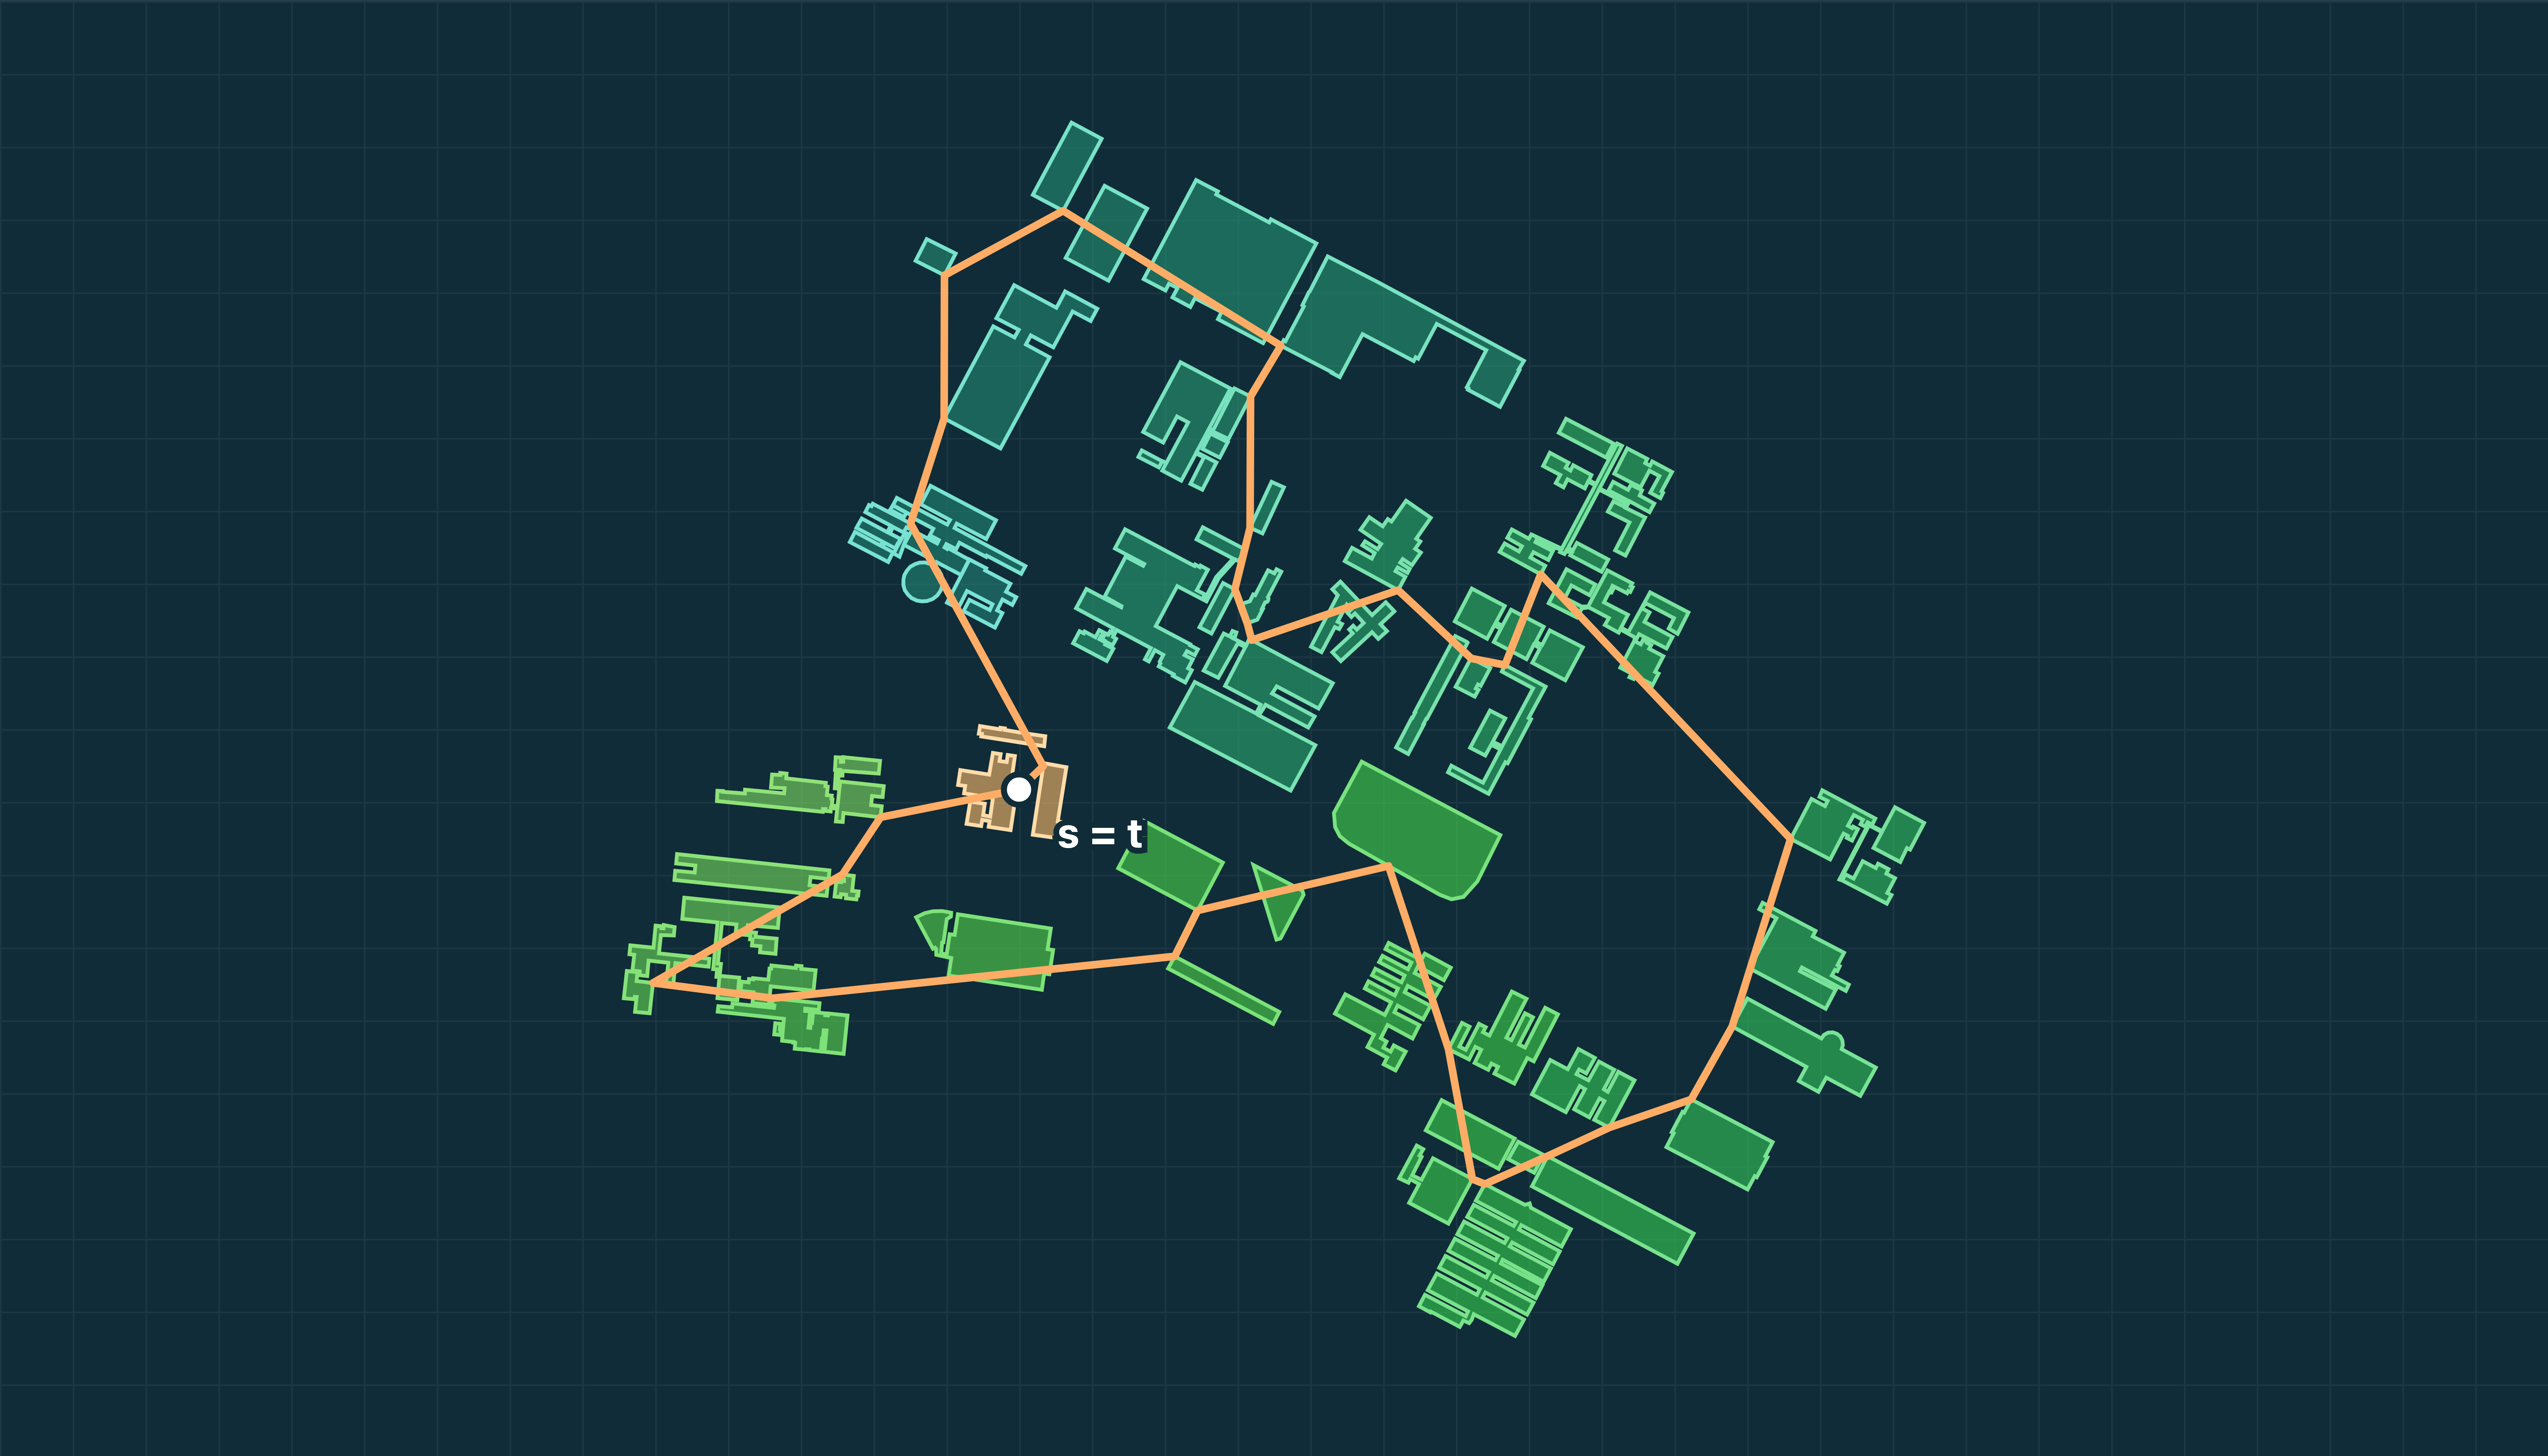
\includegraphics[width=\linewidth]{figures/usp-route-print.png}}
  % Labels occupy the empty left margin of the original app viewport.
  \block{map-regions}{4.7}{47.0}{10.1}{\sffamily\bfseries\fontsize{80}{84}\selectfont\color{white}51\par\sffamily\mdseries\fontsize{26}{32}\selectfont regiões}
  \block{map-distance}{4.7}{55.0}{10.1}{\sffamily\bfseries\fontsize{66}{74}\selectfont\color{Route}4,97\par\sffamily\mdseries\fontsize{26}{32}\selectfont\color{white}quilômetros}
  \block{map-origin}{4.7}{63.0}{9.6}{\sffamily\fontsize{24}{31}\selectfont\color{white}Saída e retorno junto ao IME\par\vspace{0.25cm}$s=t$ fixo}
  \draw[Route,line width=3pt] (3,74.0) -- (4.6,74.0);
  \block{legend-route}{5.1}{73.45}{15.5}{\smalltext Caminho calculado}
  \shade[left color=FirstVisit,right color=LastVisit] (23.6,73.75) rectangle (27.6,74.15);
  \block{legend-order}{28.2}{73.45}{25.6}{\smalltext Primeiras $\to$ últimas visitas}
  \block{map-caption}{3}{75.7}{50.8}{\smalltext Contornos desenhados pelo autor no QGIS sobre mapa-base público (OpenStreetMap). Incluem IF, IO, FAU, Geociências, Química, FFLCH, IP, ECA, FEA, Poli, Biblioteca Brasiliana, Restaurante Central, Praça dos Bancos e Google.\par\textbf{Demonstração independente do corpus experimental.}}
  % Brute-force scale, bound comparison, and the two kinds of branching.
  \block{method-head}{56.1}{40.7}{25}{\head{04}{Buscar sem enumerar}}
  \block{brute-force}{56.1}{44.0}{19.5}{\bodytext Força bruta: testar ordens e escolhas de peças convexas. Implementamos \textbf{Greene [4]} para decompor os polígonos.}
  % Schematic convex partition of an L-shaped region (not the USP geometry).
  \fill[FirstVisit!35] (77.6,44.2) -- (79.0,44.2) -- (79.0,47.2) -- (77.6,47.2) -- cycle;
  \fill[LastVisit!45] (79.0,45.9) rectangle (80.7,47.2);
  \draw[Ink,line width=1.2pt] (77.6,44.2) -- (79.0,44.2) -- (79.0,45.9) -- (80.7,45.9) -- (80.7,47.2) -- (77.6,47.2) -- cycle;
  \draw[Ink,line width=1.0pt] (79.0,45.9) -- (79.0,47.2);
  \block{partition-label}{77.1}{47.6}{4}{\sffamily\fontsize{22}{26}\selectfont\color{Muted}peças}
  \fill[Pale] (55.5,49.3) rectangle (81.1,58.0);
  \block{case-tag}{56.4}{50.1}{23.8}{\tagtext CASO 49\hspace{0.4cm}·\hspace{0.4cm}60 REGIÕES}
  \block{case-equation}{56.4}{51.8}{23.8}{\sffamily\fontsize{37}{44}\selectfont\color{Ink}$60!\prod_i p_i\approx1{,}56\times10^{117}$}
  \block{case-explanation}{56.4}{53.9}{23.8}{\smalltext combinações formais ($p_i$: peças da região $i$).\par\textbf{Resolvido em 2,47 s, com uma thread.}\par O solver não enumerou esse espaço.}
  \block{branch-and-bound}{56.1}{59.1}{25}{\bodytext No \textbf{branch-and-bound}, cada nó guarda uma ordem parcial e escolhas de fechos ou peças. Omitir visitas e usar fechos convexos relaxa o problema.}
  \block{lower-bound}{56.1}{65.5}{11.9}{\smalltext\textbf{Solver convexo}\par limite inferior $L$}
  \block{upper-bound}{69.2}{65.5}{11.9}{\smalltext\textbf{Rota completa}\par incumbente $U$}
  \draw[Muted,line width=1.4pt,-{Stealth[length=3.5mm]}] (61.8,68.1) -- (61.8,68.7) -- (67.8,68.7) -- (67.8,69.3);
  \draw[Muted,line width=1.4pt] (74.9,68.1) -- (74.9,68.7) -- (67.8,68.7);
  \block{prune}{56.1}{69.6}{25}{\centering\sffamily\bfseries\fontsize{39}{47}\selectfont\color{Accent}$L\geq U-\varepsilon\ \Rightarrow\ \text{poda}$}
  \block{branch}{56.1}{72.2}{25}{\bodytext Sem poda, inserir uma região em cada posição possível ou refinar seu fecho em peças. Integramos ordem e peças em \textbf{uma só árvore}.}
  \block{method-note}{56.1}{77.9}{25}{\smalltext Inserção e refinamento adaptados de [3]. IF $\to$ Central $\to$ IAG ilustra um desvio; só um limite válido justifica a poda.}
  % Results follow the method, with denominators and protocol beside each claim.
  \draw[Rule,line width=1.1pt] (3,81.8) -- (81.1,81.8);
  \block{results-head}{3}{82.8}{78.1}{\head{05}{Resultados no corpus de Fekete et al.}}
  \block{comparison-scope}{3}{85.4}{78.1}{\smalltext Mesmo TPP adaptado: extremos fixos, ordem livre e \textbf{uma thread por instância}. Núcleo próprio: sem Gurobi no solver convexo e sem CGAL na decomposição.}
  \block{speedup}{3}{88.2}{17.9}{\metric 5,11×\par\vspace{0.2cm}\bodytext\textbf{speedup mediano}\par\smalltext Fekete/nosso nas 550\par concluídas por ambos}
  \block{solved}{23.0}{88.2}{18.1}{\metric 558/558\par\vspace{0.2cm}\bodytext\textbf{concluídas}\par\smalltext pelo nosso solver,\par na tolerância declarada}
  \block{under-ten}{43.0}{88.2}{18.1}{\metric 477/558\par\vspace{0.2cm}\bodytext\textbf{abaixo de 10 s}\par\smalltext com o nosso solver}
  \block{faster}{63.0}{88.2}{18.1}{\metric 492/550\par\vspace{0.2cm}\bodytext\textbf{mais rápidas}\par\smalltext com o nosso solver,\par no conjunto comum}
  \block{protocol}{3}{95.0}{37.9}{\smalltext\textbf{Fekete:} 550/558 concluídas com gap relativo $\leq0{,}1\%$; rodada de 10 s e até 6 h nos remanescentes. Uma campanha; metadados completos de hardware e compilação não foram preservados.}
  \block{certificate}{43.0}{95.0}{38.1}{\smalltext\textbf{Nosso ``ótimo'':} visitas verificadas e limites globais\par $U-L\leq\varepsilon=10^{-7}+10^{-9}|U|$.\par Fechamento numérico, não aritmética exata global. O pior caso da busca permanece exponencial.}
  \block{visit-audit}{3}{99.0}{78.1}{\sffamily\mdseries\fontsize{23}{28}\selectfont\color{Muted}\textbf{Precisão das visitas:} máximo das distâncias mínimas rota--região $\leq10^{-7}$ nas unidades dos dados: nosso \textbf{558/558}; Fekete \textbf{130/551} trajetórias brutas disponíveis.}
  % Open questions and invitation to the interactive application.
  \draw[Rule,line width=1.1pt] (3,101.0) -- (81.1,101.0);
  \block{open-head}{3}{102.0}{35}{\head{06}{Questões em aberto}}
  \block{open}{3}{104.7}{35}{\sffamily\mdseries\fontsize{27}{33}\selectfont\color{Ink}\textbf{Extremos como regiões:} escolher o ponto de partida numa região, impondo $s=t$ para manter a rota fechada.\par\textbf{Menos peças:} avaliar partições com pontos de Steiner, como Chazelle--Dobkin [5], e seu custo na busca.}
  \block{app-head}{41}{102.0}{29.0}{\head{07}{Construa sua rota}}
  \block{app}{41}{104.7}{28.8}{\sffamily\mdseries\fontsize{27}{33}\selectfont\color{Ink} Tente \textbf{3 desafios} e compare suas escolhas com o ótimo certificado nas tolerâncias. Explore USP, São Paulo e Brasil, \textbf{186 registros} de busca passo a passo, dados e rotas dos \textbf{558 casos} e contatos.}
  \block{app-link}{41}{110.2}{28.8}{\sffamily\fontsize{22}{27}\selectfont\color{Muted}\href{https://yushipy.github.io/TouringPolygons/apps/siicusp34/}{yushipy.github.io/TouringPolygons/apps/siicusp34/}}
  \block{qr}{72.4}{102.7}{8.3}{\qrcode[level=H,height=8.3cm]{https://yushipy.github.io/TouringPolygons/apps/siicusp34/}}
  % References and credits; the digital PDF keeps live links.
  \draw[Rule,line width=0.8pt] (3,111.6) -- (81.1,111.6);
  \block{references-left}{3}{112.2}{32.0}{\sffamily\fontsize{22}{27}\selectfont\color{Muted}\textbf{Referências}\par
  [1] Dror et al. \href{https://doi.org/10.1145/780542.780612}{\emph{Touring a Sequence of Polygons}}. STOC, 2003.\par
  [2] Tan; Jiang. \href{https://doi.org/10.1007/978-3-319-55911-7_44}{\emph{Efficient Algorithms for Touring a Sequence of Convex Polygons and Related Problems}}. TAMC, 2017.\par
  [3] Fekete et al. \href{https://doi.org/10.4230/LIPIcs.SoCG.2026.46}{\emph{A Branch-and-Bound Algorithm for the Traveling Salesman Problem with Difficult Neighborhoods}}. SoCG, 2026.}
  \block{references-right}{37}{112.2}{28.2}{\sffamily\fontsize{22}{27}\selectfont\color{Muted}
  [4] Greene. \emph{The Decomposition of Polygons into Convex Parts}. Computational Geometry, 1983.\par
  [5] Chazelle; Dobkin. \href{https://doi.org/10.1016/B978-0-444-87806-9.50009-8}{\emph{Optimal Convex Decompositions}}. Computational Geometry, 1985.\par\vspace{0.12cm}
  \href{mailto:gabriel_ushijima@usp.br}{gabriel\_ushijima@usp.br}\quad\href{mailto:egbirgin@ime.usp.br}{egbirgin@ime.usp.br}\par
  O autor declara não haver conflito de interesses.}
  \block{funding-logo}{69.0}{113.2}{12.1}{
\includegraphics[width=\linewidth]{figures/fapesp-logo.png}}
  \block{funding}{69.0}{116.5}{12.1}{\sffamily\fontsize{22}{27}\selectfont\color{Muted}Processo 2025/13861-1}
\end{tikzpicture}
\end{document}
